\documentclass[a4paper, 12pt]{article}
\usepackage{authblk}
\renewcommand{\Affilfont}{\footnotesize}
\title{Cabinet under Pressure: Survival Analysis of Peru’s Prime Ministers Since 1980}
\author[1,2]{ Jose Manuel Magallanes}
\affil{PULSO -Institute of Social Analytics and Strategic Intelligence\thanks{The author would like to thank the research assistants from PULSO-PUCP: Alexandra Porras, Alfredo Aro, Romina Loayza, Ivana Delgado, and Bruno Mago for their support  and dedication to this work.} and Department of Social Sciences, Pontificia Universidad Catolica del Peru, San Miguel 15088, Lima, Peru}
\affil[2]{University of Massachusetts-Amherst; University of Washington -Seattle; and Universidad Nacional Mayor de San Marcos-Lima}
\affil[*]{Corresponding author: jmagallanes@pucp.edu.pe}

\usepackage{tabularx,booktabs,threeparttablex,multirow,float}
\date{\today}  %% manually: \date{March 6, 2025} 
\usepackage[natbibapa]{apacite} %% for bibliography
\usepackage{rotating, graphicx} %% for rotating tables
\usepackage{adjustbox} % size of plots and tables
\usepackage{chngcntr}% section numbering
\usepackage{amssymb}
\usepackage{threeparttable}
\usepackage[table]{xcolor}
\usepackage{longtable}
\usepackage{array}        % For raggedright column specifier
\counterwithin{table}{section}\counterwithin{figure}{section}
\usepackage{Sweave}
\begin{document} % every "begin: needs and "end"
\Sconcordance{concordance:premieres.tex:premieres.Rnw:1 21 1 1 0 153 1 1 26 18 0 1 2 %
230 1 1 12 29 0 1 2 270 1}

\maketitle 
\begin{abstract}
This study examines the political durability of Peru’s Prime Ministers (Presidente del Consejo de Ministros, PCM) since the country’s democratic return in 1980. Using survival analysis, we explore how political context, institutional conditions, and crisis dynamics shape the tenure of these key presidential appointees. Through a Cox proportional hazards model, we test the influence of presidential popularity, legislative fragmentation, cabinet reshuffles, and regime instability on the risk of early dismissal or resignation. The results illuminate how informal power-sharing and institutional fragility influence executive coordination in a hyper-presidential regime.
\end{abstract}




\section{Introduction} % * to unnumber

Although the 1979 Constitution of Peru defined the Prime Minister (PCM) merely as the president’s first minister—responsible for countersigning decrees and coordinating cabinet activity—subsequent legal and political developments have elevated the office to one that routinely performs head-of-government functions. These include drafting the policy agenda, negotiating confidence votes, and representing the executive in congressional interpellations. The PCM has thus come to serve as the president’s chief political shield. In periods of stable governance, the office facilitates legislative compromise and projects technocratic competence; in times of crisis, it functions as a “circuit-breaker”—a high-visibility scapegoat whose dismissal absorbs congressional discontent and helps preserve presidential tenure. Analyzing the determinants of PCM survival therefore sheds light on how Peru’s hyper-presidential system manages accountability, blame attribution, and policy coordination in the absence of strong political parties.
\begin{figure}[ht]
\centering
% \begin{adjustbox}%{width=0.9\textwidth,height=12cm,clip,trim=0cm 0cm 0cm 0cm} 
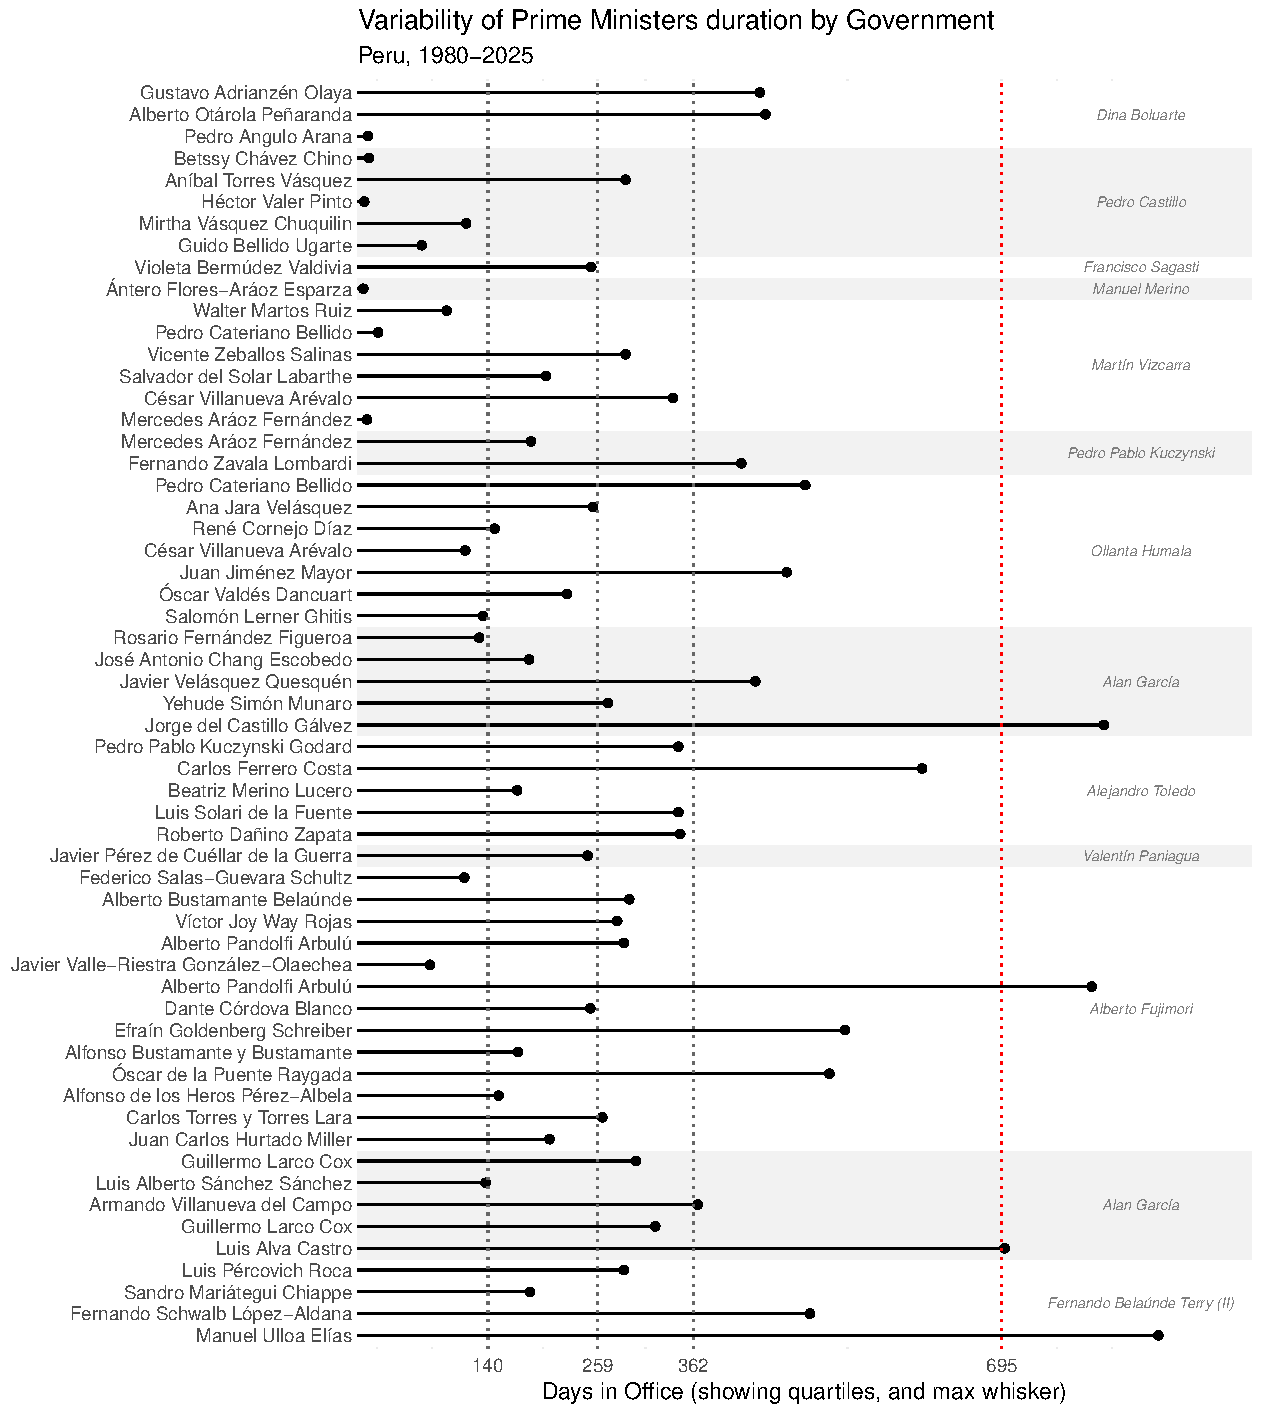
\includegraphics[width=0.85\textwidth]{durationLolli.pdf}
% \end{adjustbox}
\caption{Variability and Statistics Duration of PCMs in Perú from 1980 until 2025}  
\label{durationLolli} 
\end{figure}

The significance of this institutional role is underscored by the striking variation in PCM tenures. The median tenure since 1980 is just 254 days (approximately eight months), but durations vary widely (see Figure~\ref{durationLolli}). Ántero Flores-Aráoz lasted only six days in November 2020, whereas Manuel Ulloa served 864 days in the early 1980s, and Jorge del Castillo remained in office for 805 days during Alan García’s second term. This volatility persists even within single presidential administrations: three PCMs held the post during Pedro Castillo’s first five months, while Alberto Otárola remained in office for 440 days under Dina Boluarte. 

\begin{figure}[ht]
\centering
% \begin{adjustbox}%{width=0.9\textwidth,height=12cm,clip,trim=0cm 0cm 0cm 0cm} 
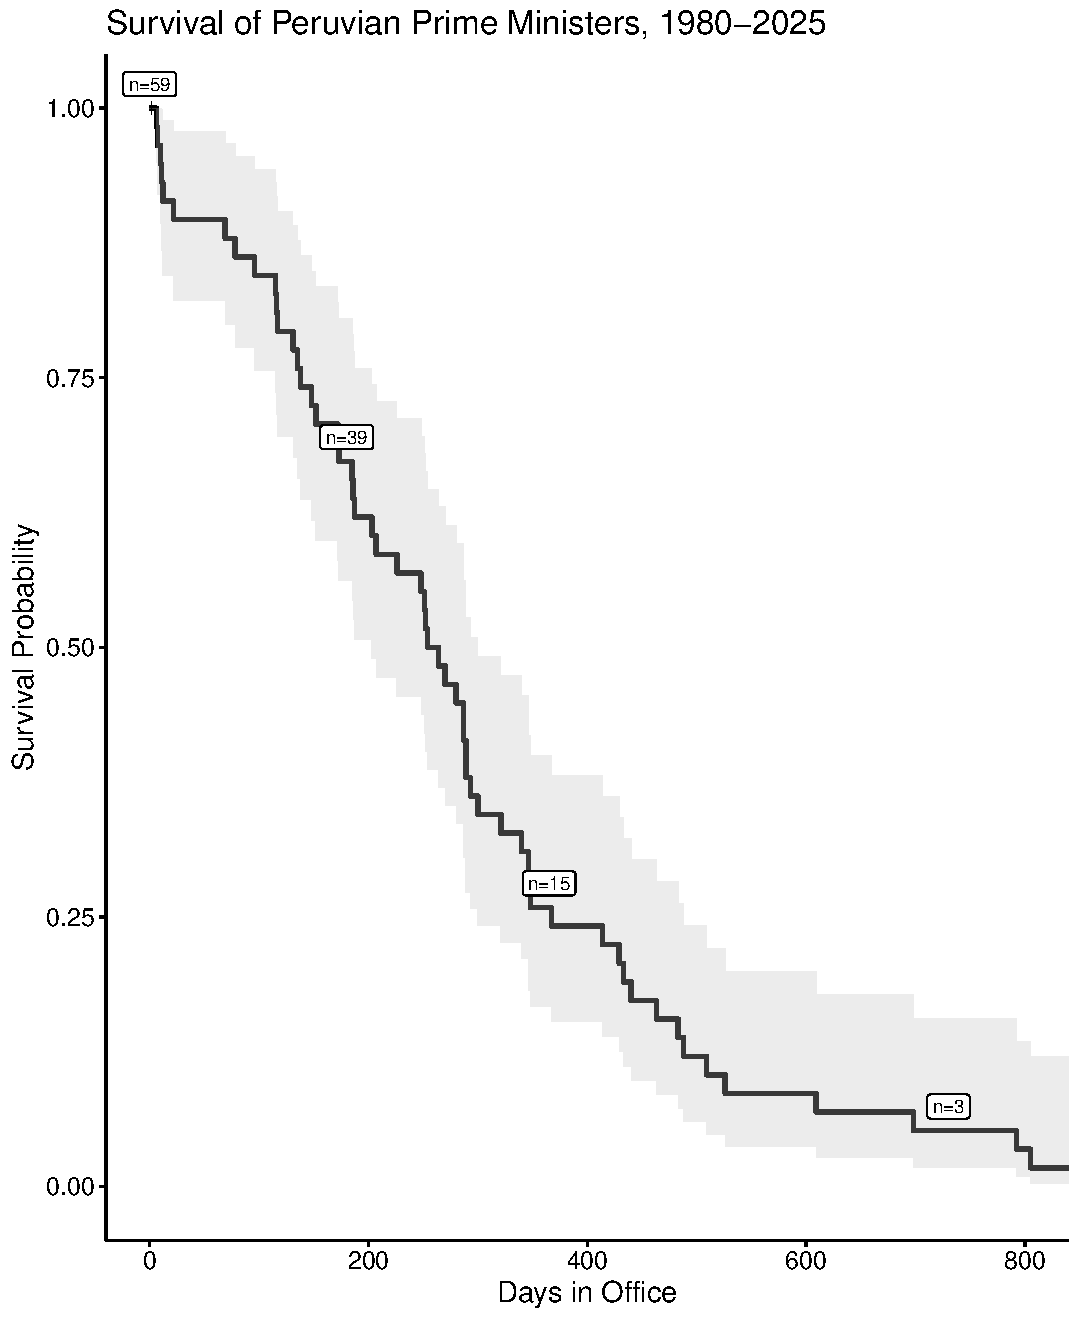
\includegraphics[width=0.85\textwidth]{kaplanDuration.pdf}
% \end{adjustbox}
\caption[Survival of Prime Ministers in Peru]{Kaplan-Meier survival estimate for Peruvian Prime Ministers, 1980--2025.}
\label{kaplanDuration} 
\end{figure}

The Kaplan-Meier survival estimate (Figure \ref{kaplanDuration}) illustrates this volatility. At the outset, all 58 PCMs are at risk. Within six months, only 40 remain; by one year, just 30 are still in office, and by the two-year mark, this number falls to 17. The survival probability drops below 50\% well before the one-year point and declines to around 20\% by year two. This pattern highlights how short-lived PCM tenures have become a structural feature of Peru’s political system rather than a sign of exceptional disruption. Understanding the forces behind such high turnover thus requires systematic analysis of the political, institutional, and situational factors that shape PCM survival—an inquiry taken up in the remainder of this study. Such inconsistency—despite ostensibly stable institutional rules—raises a central puzzle: which political, institutional, and situational factors shape the durability of Peru’s Prime Ministers?



\section{Background}\label{backg-tables} % label for crossref

\subsection{Evolution of the Prime Minister’s formal mandate} Peru’s Prime Minister (PCM) has migrated from a cabinet chair of convenience in the 1979 Constitution to a multisector policy coordinator and modernisation czar under the post‑2000 statutory framework.  Four legal milestones define that trajectory:


\begin{itemize}
\item 1979 Constitution (arts.215–218). The PCM presides over the Council of Ministers only when the President is absent; all appointments and dismissals rest with the President, who may chair the Council at will.  The PCM’s core duty is to secure majority support inside the cabinet for bills, decree‑laws, and matters of public interest. (Constitution 1979.)

\item 1993 Constitution (arts. 122–127). Retains presidential discretion over appointments but upgrades the PCM: he/she convenes the Council, signs legislative decrees, and must present the government programme and request a vote of confidence from Congress. (Democratic Constituent Congress 1993.)
\item Organic Law of the Executive Branch – LOPE 2007 (ch. II). Charges the PCM with proposing the government’s general objectives, coordinating multisectoral national policies—especially economic and social development—and supervising entities attached to the Presidency of the Council of Ministers. (Congress of the Republic 2007, LOPE.)
\item Law 29158 (2007) on Modernisation of the State (art.19). Designates the PCM the President’s highest‑trust agent, responsible for steering public‑sector modernisation and decentralisation across all tiers of government.  (Congress of the Republic 2007, Law 29158.)
\end{itemize}

Together these reforms turned the PCM from symbolic countersignatory into the President’s principal political shield and agenda gate‑keeper. See Table \ref{tab:pcm-mandate} for details on this evolution.

\begin{sidewaystable}[p]   % ‘p’ = put on its own float page
\centering
\caption{Evolution of the PCM’s formal mandate since 1979}
\label{tab:pcm-mandate}
\renewcommand{\arraystretch}{1.2}
\begin{tabularx}{\textheight}{@{}l X X X X l@{}}  % \textheight fits the rotated width
\toprule
\textbf{Legal framework} &
\textbf{Cabinet-chair role} &
\textbf{Policy-coordination powers} &
\textbf{Appointment \& dismissal} &
\textbf{Additional statutory duties} &
\textbf{Citation}\\
\midrule
1979 Constitution &
Chairs Council only when President absent; President may chair at will &
Secures majority consent for bills and decree-laws within the cabinet &
Exclusive presidential prerogative &
None specified beyond cabinet deliberations &
Const.\ 1979, arts.\ 215–218\\[4pt]

1993 Constitution &
Convenes Council; President may still chair &
Countersigns decrees; presents programme and confidence motion to Congress &
Exclusive presidential prerogative &
Must seek confidence votes &
Const.\ 1993, arts.\ 122–127\\[4pt]

LOPE 2007 &
PCM regularly chairs Council (President rarely attends) &
Proposes government objectives; coordinates multisector policies; supervises PCM-attached entities &
Unchanged &
Broad multisector supervision &
LOPE 2007, ch.\ II\\[4pt]

Law 29158 (2007) &
As per LOPE &
Leads State modernisation and decentralisation agenda &
Unchanged &
Strategic planning; inter-governmental coordination &
Law 29158, art.\ 19\\
\bottomrule
\end{tabularx}
\end{sidewaystable}

\subsection{Informal evolution: from symbolic coordinator to political operator}

The Prime Minister’s day‑to‑day leverage has always depended less on parchment rules than on shifting presidential strategies and congressional configurations.  Three sequential informal models can be distinguished:

\begin{itemize}

\item Symbolic coordinator (1980–1990).Under Belaunde and the first García administration the PCM remained a low‑profile chair; party‑fragmented congresses preferred dealing directly with sector ministers, and premiers changed whenever coalition arithmetic shifted.  Average tenure was 405 days, but the post was still viewed as an honorific stepping‑stone rather than a power centre.

\item Gate‑keeper in an autocratic presidency (1990 – 2000). Fujimori’s autogolpe (1992) sidelined Congress and broadened decree‑law rule.  The PCM became the sole bureaucratic filter for emergency economic decrees and IMF‑negotiated reforms; loyalty trumped expertise (e.g., Hurtado Miller, Pandolfi).  Although the decade’s mean tenure fell to $\approx 302$ days, variance shrank because Fujimori kept loyalists long until a policy pivot required a full cabinet refresh.

\item Floor‑manager and lightning rod (2001 – present). With the 1993 Constitution’s confidence‑vote mechanism now routinised, the PCM took on vote counting and crisis‑absorption roles.

\begin{itemize}

\item Coalition minority years (Toledo 2001‑06): premiers (e.g., Carlos Ferrero) traded ministerial posts for legislative backing.  

\item Party‑government years (García II 2006‑11): Jorge del Castillo doubled as APRA whip, illustrating the PCM’s partisan link function.  
\item Confrontational years (PPK, Vizcarra, Castillo): Congress weaponised interpellations; presidents sacrificed PCMs (Zavala 2017; Villanueva 2018; Bellido→Vásquez→Torres 2021‑22) to defuse censure threats or reset talks before the 28 July speech.  

\item Post‑2022 caretaker presidency: Dina Boluarte retained Alberto Otárola for 440 days to project continuity amid unrest, showing the PCM as stability signal.
\end{itemize}
\end{itemize}


Across these phases, two informal prerogatives emerged:

\begin{itemize}
\item Negotiator‑in‑chief. Modern PCMs draft the annual Mensaje a la Nación, map votes for confidence motions, and lobby party spokespeople—tasks never spelled out in LOPE.

\item High‑visibility “circuit‑breaker.” Presidents now time reshuffles to absorb blame for corruption scandals (e.g., Saavedra 2016 education dispute; Chávarry 2019 judicial scandal) or economic shocks, banking on a short‑term boost in approval.

\end{itemize}

These unwritten practices explain why Prime‑Ministerial exits cluster around scandals, protests, and the July speech window—patterns the survival analysis in Section 4 explicitly models.


\subsection{Prime‑Ministerial tenure across political periods}

Peru’s Prime‑Ministerial tenure remains volatile, but volatility itself is not uniform across eras.  Using the verified dataset of 57 spells (1980–2025), Table \ref{tab:durationPerEra} summarises the distribution by political period.  The Fujimori decade exhibits the shortest average tenure (302 days) yet also the narrowest spread, reflecting the concentration of presidential power; the immediate post‑transition years average roughly 405 days, while the post‑2000 era shows the shortest median (232 days) and the widest range as presidents cycle through PCMs to manage fragmented congresses and serial crises.



\begin{table}[!h]
\centering
\caption{Duration in Days by era\label{tab:durationPerEra}}
\centering
\begin{threeparttable}
\begin{tabular}[t]{lrrrrr}
\toprule
Era & count & mean & min & max & range\\
\midrule
A. Belaunde to Garcia & 9 & 405.44 & 138 & 864 & 726\\
B. Fujimori & 13 & 302.08 & 78 & 792 & 714\\
C. Paniagua to Boluarte & 36 & 247.56 & 6 & 805 & 799\\
\bottomrule
\end{tabular}
\begin{tablenotes}[para]
\item \textit{Source: } 
\item author calculations from official appointment resolutions and El Peruano archives.
\end{tablenotes}
\end{threeparttable}
\end{table}

\section{Literature Review}\label{sec:letrev}

The formal mandate outlined in Table \ref{tab:pcm-mandate} establishes the PCM as the president’s chief policy coordinator and political shield. The subsections that follow review comparative findings on the political, institutional, and situational determinants of ministerial tenure, providing the theoretical backdrop for our hypotheses.


\subsection{Cabinet Volatility in Peru}

Early comparative work portrays Peru as an extreme case of ministerial churn.  \citet{martinez-gallardo_out_2012} reports an average cabinet duration of just 13 months (1980–2000), less than half the Latin‑American mean and exceeded only by Brazil.  Sector‑specific studies corroborate the pattern: in the health ministry, average tenure was 13.7 months between 1935 and 2021 \citep{gozzer_duracion_2021}.  Frequent reshuffles reset reform agendas—“policies are often returned to square one” \citealp[335]{gozzer_duracion_2021} —and cascade through lower administrative layers.  Yet the causes of this volatility remain under‑specified.

\subsection{Critical Events and Shocks}

Extant research highlights critical events as proximate triggers of turnover.  \citet{dewan_corrective_2005} show that UK prime ministers reshuffle after scandals to restore popularity; \citet{camerlo_minister_2015-1} find media scandals and social protests heighten rotation in twelve Latin‑American democracies, with effects conditioned by the electoral calendar and re‑election rules.  Because Peruvian presidents cannot be re‑elected, the country fits Camerlo and Pérez‑Liñán’s scenario in which protests spike hazard early in the term, while scandals matter later \citet[616]{camerlo_minister_2015-1}. Economic crises operate similarly: \citet{gonzalez-bustamante_cambios_2016} incorporate downturns into Chilean survival models, and \citet[515]{fischer_duration_2012} argue that a minister’s post‑shock fate hinges on formal removal rules, political weight, and net benefit to the government.


\subsection{Institutional Determinants}

Turning to institutional factors, the presidential–parliamentary divide looms large.
From \citet{fischer_duration_2012} we learned that Single-party cabinets generally stay in power longer than coalitions; within coalitions, minimum-winning cabinets outlive surplus (oversized) coalitions; Cabinets endure markedly longer in parliamentary systems\footnote{Blondel’s cross-national data show presidential cabinets are the shorter-lived side of the divide \citep{blondel_government_1985}}. If the regime were authoritarian, cabinets in communist regimes lived longer than the ones from military dictatorships; and finally, Cabinets with more veto-player parties are less durable.

Some of those findings complement the ones above.  A sixty‑year study of Colombia shows that multiparty coalition presidentialism lengthens tenure, whereas two‑party periods display higher churn \citep{mejia_es_2021}.  Uruguay’s above‑average stability likewise hinges on durable coalitions; crises coincide with coalition breakdowns \citep{chasquetti_designacion_2013}.


\subsection{Ministerial Profiles}

Personal attributes cannot be ignored.  Age effects are U‑shaped, with the youngest and oldest ministers more likely to exit \citet{fischer_duration_2012}.  \citet{escobar-lemmon_coming_2010} find that being in the inaugural cabinet and holding the finance portfolio increase hazard, whereas constituency links reduce it.  Prior political experience, however, has only marginal impact \citep{escobar-lemmon_coming_2010}.  In Peru, outsider presidents such as Alberto Fujimori and Pedro Pablo Kuczynski have consistently favoured technocrats with scant partisan capital \citep{carreras_presidentes_2013,nercesian_radiografigabinetes_2019}.  Whether such technocratic cabinets enjoy longer—or shorter—survival remains an open empirical question.

To empirically assess whether technocratic traits influence PCM survival, we model the technocratic profile as a latent trait composed of five binary indicators drawn from comparative literature: absence of prior electoral participation, foreign graduate education, private sector experience, academic engagement, and having a degree other than law. These attributes are commonly cited as markers of technocratic identity 
\citep{carreras_presidentes_2013,alexiadou_commitment_2019,alexiadou_ideologues_2015,escobar-lemmon_coming_2010}. Rather than selecting a single proxy, we construct a latent index using latent trait modeling (LTM), which estimates each PCM’s position on the technocratic dimension. This method aligns with recent work on ministerial professionalism \citep{bersch_state_2017} and allows us to capture degrees of technocratic orientation rather than impose a binary categorization. We validate this index using exploratory factor analysis and principal components, both of which confirm a consistent underlying dimension.

% 

\subsection{Gaps in the Literature and Relevance to Peru}

Existing studies converge on three explanatory families—critical events, institutional arrangements, and individual profiles—but seldom test them jointly inside a single presidential system.  Moreover, most Latin‑American research pools multiple countries, obscuring Peru’s idiosyncrasies: (i) constitutional hyper‑presidentialism without the stabilising force of strong parties; (ii) the annual Mensaje a la Nación on 28 July, a focal point for reshuffles; and (iii) recurrent economic volatility.  By integrating LOPE’s formal mandates with comparative findings on shocks, institutions, and minister profiles, the present study builds a tailored framework for explaining why some Peruvian PCMs become expendable “circuit‑breakers” while others endure.



\section{Data and Methods}

\subsection{Dataset construction}


This study draws on an event-history dataset covering all 57 Prime-Ministerial spells between 28 July 1980 and 8 May 2025. Each spell corresponds to a continuous period during which a single individual served as Prime Minister (PCM), from their swearing-in to dismissal or resignation. Gustavo Adrianzén’s ongoing tenure is treated as right-censored as of 8 May 2025.

The explanatory variables are grouped into two categories:

\textbf{(a) Non–time-varying variables}, which remain constant throughout a PCM’s spell. These include:

\begin{itemize}
    \item \textit{Technocratic profile}: A latent trait index derived from five binary indicators: (i) absence of previous electoral participation, (ii) graduate degree obtained abroad, (iii) relevant private sector experience, (iv) academic background, and (v) having a degree other than law. These variables reflect the literature on technocratic appointments (Carreras, 2013; Alexiadou, 2016; Escobar-Lemmon \& Taylor-Robinson, 2010). We estimate a continuous score using Latent Trait Modeling (LTM), validated through PCA and EFA. The continuous index is used in all Cox regressions; a binary split at the median is used for descriptive survival plots.
    
    \item \textit{Fujimori regime dummy}: A fixed indicator for spells that occurred during the presidency of Alberto Fujimori (April 1990 to July 2000), capturing the autocratic institutional context of that period.
\end{itemize}

\textbf{(b) Time–varying variables}, which may change within a PCM’s tenure and thus require finer temporal resolution. These include:

\begin{itemize}
    \item \textit{Presidential approval}: Quarterly approval ratings from Ipsos Perú;
    \item \textit{Legislative fragmentation}: Measured via the effective number of parties (ENP), calculated from congressional seat shares;
    \item \textit{Censure motions}: A binary indicator coded 1 if a motion for interpellation or censure was active during the interval;
    \item \textit{Economic shock}: Equals 1 if quarterly GDP growth is negative;
    \item \textit{Speech window}: Equals 1 if the interval includes ±45 days around the annual \textit{Mensaje a la Nación} on 28 July.
\end{itemize}

To correctly update these time-varying covariates mid-tenure, we adopt the Andersen–Gill (AG) counting-process framework, splitting each PCM spell into annual intervals anchored on 28 July. This allows each time-varying covariate to update in a temporally valid way while preserving the structure of the Cox partial likelihood. Robust standard errors are clustered by PCM to account for repeated observations.

\begin{sidewaystable}[p]
\scriptsize
\centering
\caption{Variables, Operationalization, Sources, and Literature}
\label{tab:variables}
\begin{tabular}{
  >{\raggedright\arraybackslash}p{3cm} 
  >{\raggedright\arraybackslash}p{3.5cm} 
  >{\raggedright\arraybackslash}p{6cm} 
  >{\raggedright\arraybackslash}p{2.5cm} 
  >{\raggedright\arraybackslash}p{4cm}
}
\toprule
\textbf{Category} & \textbf{Variable} & \textbf{Operationalization} & \textbf{Source} & \textbf{Literature} \\
\midrule

\multicolumn{5}{l}{\textit{Non–Time-Varying Covariates}} \\
\midrule

Profile & Technocrat Index & Latent trait score from five binary indicators: no electoral experience, foreign graduate education, private sector or academic background, and non-law degree. Estimated via LTM and validated via PCA and EFA. & CVs and secondary sources & Carreras (2013); Alexiadou (2016); Escobar-Lemmon \& Taylor-Robinson (2010); Bersch et al. (2017) \\

Regime & Fujimori & 1 if PCM served between 5 April 1990 and 28 July 2000 & Author coding & Pérez-Liñán (2007); Fischer et al. (2012) \\

\midrule
\multicolumn{5}{l}{\textit{Time–Varying Covariates}} \\
\midrule

Congress & ENP & Quarterly effective number of parties (seat share) & JNE seat records & Huber \& Martínez-Gallardo (2008); Martínez-Gallardo (2012) \\

Congress & Censure motion & 1 if interpellation or censure motion was tabled during interval & Congressional Journal & Camerlo \& Pérez-Liñán (2015); Dewan \& Dowding (2005) \\

Presidency & Approval & Quarterly presidential approval (\%) & Ipsos Perú & Samuels \& Shugart (2003); Fischer et al. (2012) \\

Calendar & Speech window & 1 if within ±45 days of 28 July & Author calculation & This study (informal calendar logic) \\

Economy & GDP shock & 1 if quarterly GDP growth is negative & BCRP & González-Bustamante \& Olivares (2016) \\

\bottomrule
\end{tabular}
\end{sidewaystable}



%%%

\subsection{Computing Time Invariant Covariates}

\subsubsection{The regime epoch}

\subsubsection{Latent Trait Modeling of Technocratic Profile}

To operationalize the technocratic orientation of Prime Ministers (PCMs), we estimate a latent trait model using three binary indicators grounded in the literature on technocratic appointments in Latin America and beyond: (i) absence of prior electoral participation, (ii) possession of a graduate degree from a foreign university, and (iii) relevant private sector experience. Each trait captures a distinct aspect of the technocratic profile.

The absence of electoral participation reflects political independence, a hallmark of technocratic appointments, particularly under outsider presidencies and in contexts of weak party institutionalization \citep{escobar-lemmon_coming_2010, carreras_presidentes_2013}. A foreign graduate degree signals technical training and elite socialization, often aligned with global policy norms \citep{alexiadou_ideologues_2016, camp_mexicos_2002}. Private sector experience, particularly in consulting, banking, or corporate management, signals not only managerial competence but also autonomy from state careers. Technocrats often derive their legitimacy from reputational capital earned outside the public sector. As Alexiadou and Günaydin \citep{alexiadou_commitment_2019} argue, technocrats are professionals motivated by expertise and external reputation, who “typically aim at better employment prospects by building a positive reputation in their professional field.” This complements Dargent’s \citep{dargent_technocracy_2014} observation that many Latin American technocrats enter the state from positions of market-based credibility rather than political dependence. Similar arguments are found in earlier studies linking private sector expertise to technocratic authority in reform-oriented administrations \citep{centeno_democracy_1997, weyland_politics_2021}.

We model these three traits as manifestations of a continuous latent technocratic dimension using a two-parameter logistic latent trait model (2PL), estimated with the \texttt{ltm} package in R. The model allows for item-specific variation in difficulty and discrimination, and assumes that the probability of endorsing each trait increases with the unobserved technocratic score.

As you can see in Table \ref{tab:ltm_parameters}, estimation results show that “no prior electoral experience” and “foreign graduate degree” are strong discriminators (discrimination parameters > 2.1), while “private sector experience” has lower discrimination (1.17) but higher difficulty (0.91), suggesting it marks the upper end of the technocratic scale. Figure \ref{fig:iccplot} presents item characteristic curves (ICCs) for the three indicators.

Individual-level scores are computed using expected a posteriori (EAP) estimation and assigned to PCMs by matching response patterns to model-derived scores. The resulting technocratic index ranges from approximately --1.5 to +2.6, with higher scores reflecting stronger technocratic profiles. The index is strongly correlated with PCA- and EFA-based indices ($r > 0.95$), and tracks well with clusters identified via unsupervised classification.

The continuous LTM-based index is used in Cox proportional hazards models to assess its effect on PCM survival. For descriptive Kaplan–Meier analysis, we also construct a binary version based on the median split.

% latex table generated in R 4.4.0 by xtable 1.8-4 package
% Thu May 15 19:42:25 2025
\begin{table}[ht]
\centering
\caption{Latent Trait Model: Discrimination and Difficulty Parameters} 
\label{tab:ltm_parameters}
\begin{tabular}{lrrrc}
  \hline
Parameter & Estimate & Std. Error & z-value &  \\ 
  \hline
\addlinespace
\multicolumn{4}{l}{\textit{Discrimination Parameters}} \\[-15pt] &  &  &  &  \\ 
  No electoral participation & 2.18 & 1.62 & 1.35 &  \\ 
  Foreign degree & 2.16 & 1.57 & 1.37 &  \\ 
  Private sector experience & 1.20 & 0.64 & 1.87 & . \\ 
  \addlinespace
\multicolumn{4}{l}{\textit{Difficulty Parameters}} \\[-15pt] &  &  &  &  \\ 
  No electoral participation & 0.30 & 0.23 & 1.27 &  \\ 
  Foreign degree & 0.49 & 0.26 & 1.87 & . \\ 
  Private sector experience & 0.92 & 0.44 & 2.07 & * \\ 
   \addlinespace
\addlinespace
\multicolumn{5}{l}{\footnotesize\textit{Model fit: log-likelihood = -97; AIC = 205.02; BIC = 216.95.}} \\\multicolumn{5}{l}{\footnotesize\textit{Estimated via BFGS optimization.}} \\\multicolumn{5}{l}{\footnotesize\textit{Convergence: Yes (grad = 0.00055906).}} \\\multicolumn{5}{l}{\footnotesize\textit{Integration: Gauss-Hermite with 21 points.}} \\\hline 
 \multicolumn{5}{l}{\textit{Note}: $^{*} p<0.05$, $^{.} p<0.10$} \\ 
 \hline
\end{tabular}
\end{table}


\begin{figure}[ht]
\centering
% \begin{adjustbox}%{width=0.9\textwidth,height=12cm,clip,trim=0cm 0cm 0cm 0cm} 
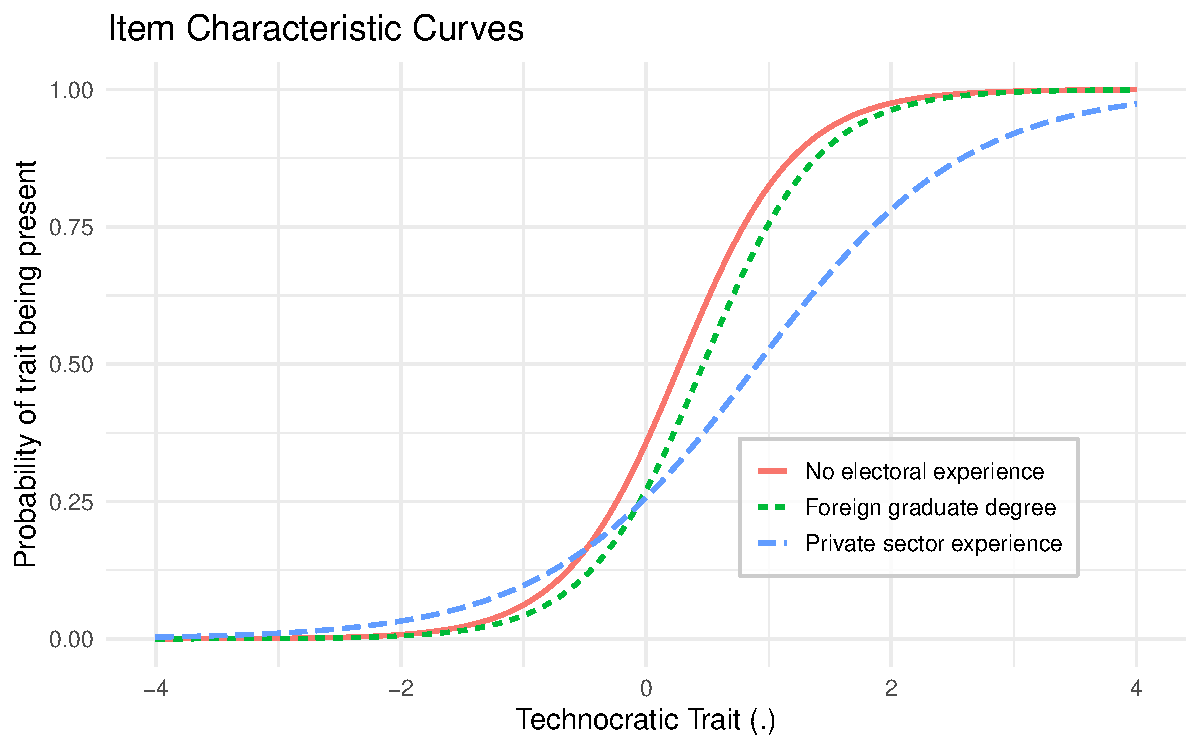
\includegraphics[width=\textwidth]{iccplot.pdf}
% \end{adjustbox}
\caption{Variability and Statistics Duration of PCMs in Perú from 1980 until 2025}  
\label{fig:iccplot} 
\end{figure}



\subsection{Model specification}

The baseline estimation is a Cox proportional‑hazards model with shared frailty by presidential administration. Ties are handled with the Efron method, and robust standard errors are clustered on presidencies to absorb unobserved style differences.

We express the hazard for PCM spell \(i\) under president \(j\) at time \(t\) as:

\[
  h_{ij}(t \mid X_i(t), u_j)
    = h_0(t) \exp\bigl(\beta^{\mathsf{T}}X_i(t) + u_j\bigr),
  \quad u_j \sim \mathcal{N}(0,\sigma^2),
\]


\paragraph{Explanation of terms}
\begin{itemize}
  \item $h_{ij}(t \mid X_i(t), u_j)$: the hazard rate for spell $i$ under president $j$ at time $t$, i.e., the instantaneous risk of exit.
  \item $h_0(t)$: the baseline hazard function, representing the underlying risk when all covariates are zero.
  \item $X_i(t)$: the vector of (possibly time-varying) covariates for spell $i$, including ENP, approval, GDP shocks, and the speech-window dummy.
  \item $\beta$: the vector of regression coefficients quantifying each covariate’s effect on the log-hazard.
  \item $\beta^\top X_i(t)$: the linear predictor (log-relative hazard) combining covariates and coefficients.
  \item $u_j$: the shared-frailty term (a random effect) for administration $j$, capturing unobserved presidency-level heterogeneity.
  \item $u_j \sim \mathcal{N}(0,\sigma^2)$: indicates $u_j$ follows a normal distribution with mean 0 and variance $\sigma^2$, where $\sigma^2$ measures unexplained variance across presidencies.
\end{itemize}


% The baseline estimation is a **Cox proportional‑hazards model with shared frailty by presidential administration**, implemented in R with the `coxme` package. Note that while `survival::coxph` supports simple frailty terms, the `coxme` package is required for estimating mixed‑effects Cox models with normally distributed random effects (shared frailty) across presidencies.








\section{Results}

% latex table generated in R 4.4.3 by xtable 1.8-4 package
% Thu May 15 14:53:41 2025
\begin{table}[ht]
\centering
\begin{tabular}{rrrrrr}
  \hline
 & coef & exp(coef) & se(coef) & z & p \\ 
  \hline
regimeFujimori & 0.02 & 1.02 & 0.37 & 0.05 & 0.96 \\ 
  technocrat\_trait\_ltm & -0.02 & 0.98 & 0.20 & -0.11 & 0.91 \\ 
   \hline
\end{tabular}
\end{table}


% 
% \subsection{Initial model}
% 
% <<echo=FALSE,results=tex>>=
% 
% library(survival)
% library(coxme)
% library(stargazer)
% # library(arrow)
% 
% 
% # 1. Load the AG intervals
% intervals_AG=arrow::read_parquet(file = "AG_intervals.parquet")
% 
% # 2. Fit the minimal “base” model: regime + speech, frailty by president
% fit_base_AG <- coxme(
%   Surv(interval_duration, event) ~ regime_fujimori + speech_window + (1 | presidentofExecutive),
%   data = intervals_AG,
%   ties = "efron"
% )
% fit=fit_base_AG
% s=summary(fit_base_AG)
% 
% 
% # --- Random effect ---
% # --- Random Effects ---
% re_sd <- round(s$random[["sd"]][1], 5)
% re_var <- round(re_sd^2, 8)
% 
% # --- Random Effects Model Fit (from s$chi) ---
% chi_df <- round(as.data.frame(s$chi), 4)
% 
% # chi_df rows: "Integrated", "Penalized"; columns: Chisq, df, p, AIC
% 
% # --- Full Model Fit ---
% loglik_val <- round(logLik(fit)[1], 2)
% df_val     <- attr(logLik(fit), "df")
% aic_val    <- round(AIC(fit), 2)
% 
% # --- Fixed Effects ---
% fe <- s$coefficients
% fe_out <- apply(fe, 1, function(row) {
%   coef <- round(row["coef"], 4)
%   hr   <- round(exp(row["coef"]), 4)
%   se   <- round(row["se(coef)"], 4)
%   z    <- round(row["z"], 2)
%   pval <- round(2 * (1 - pnorm(abs(z))), 3)
%   sprintf("%s & %.4f & %.4f & %.4f & %.2f \\quad %.3f \\\\", 
%           rownames(fe)[which(fe[, "coef"] == row["coef"])],
%           coef, hr, se, z, pval)
% })
% 
% # --- Output LaTeX file ---
% out_file <- "coxme_summary.tex"
% 
% cat(
% "\\begin{table}[ht]
% \\centering
% \\begin{threeparttable}
% \\caption{Cox Mixed-Effects Model Summary}
% \\label{tab:coxme_auto}
% \\begin{tabular}{lllll}
% \\toprule
% \\multicolumn{5}{l}{\\textbf{Random Effects}} \\\\
% \\midrule
% Group & Variable & SD & Variance & \\\\
% presidentofExecutive & Intercept & ", re_sd, " & ", re_var, " & \\\\
% \\\\
% \\multicolumn{5}{l}{\\textbf{Random Effects Model Fit (LRT)}} \\\\
% \\midrule
% Method & Chisq & df & p & AIC \\\\
% Integrated loglik & ", chi_df[1, "Chisq"], " & ", chi_df[1, "df"], " & ", chi_df[1, "p"], " & ", chi_df[1, "AIC"], " \\\\
% Penalized loglik & ", chi_df[2, "Chisq"], " & ", chi_df[2, "df"], " & ", chi_df[2, "p"], " & ", chi_df[2, "AIC"], " \\\\
% \\\\
% \\multicolumn{5}{l}{\\textbf{Full Model Fit}} \\\\
% \\midrule
% Statistic & & & & \\\\
% Penalized log-likelihood & & & & ", loglik_val, " \\\\
% Degrees of freedom & & & & ", df_val, " \\\\
% AIC & & & & ", aic_val, " \\\\
% \\\\
% \\multicolumn{5}{l}{\\textbf{Fixed Effects}} \\\\
% \\midrule
% Variable & Coef & exp(Coef) & SE(Coef) & z \\quad p \\\\
% ", paste(fe_out, collapse = "\n"), "
% \\bottomrule
% \\end{tabular}
% \\begin{tablenotes}
% \\footnotesize
% \\item \\textit{Note}: Coefficients are from a Cox proportional hazards mixed-effects model with a random intercept. SD = standard deviation of random effect. Variance = SD\\textsuperscript{2}.
% \\item \\textit{exp(Coef)} is the hazard ratio. p-values are based on z-tests.
% \\item Significance: * p<0.1; ** p<0.05; *** p<0.01
% \\end{tablenotes}
% \\end{threeparttable}
% \\end{table}
% ", file = out_file)
% 
% @
% 
% \begin{table}[ht]
\centering
\begin{threeparttable}
\caption{Cox Mixed-Effects Model Summary}
\label{tab:coxme_auto}
\begin{tabular}{lllll}
\toprule
\multicolumn{5}{l}{\textbf{Random Effects}} \\
\midrule
Group & Variable & SD & Variance & \\
presidentofExecutive & Intercept &  0.01999  &  0.0003996  & \\
\\
\multicolumn{5}{l}{\textbf{Random Effects Model Fit (LRT)}} \\
\midrule
Method & Chisq & df & p & AIC \\
Integrated loglik &  1.4  &  3  &  0.7061  &  -4.6  \\
Penalized loglik &  1.43  &  2.02  &  0.4919  &  -2.6  \\
\\
\multicolumn{5}{l}{\textbf{Full Model Fit}} \\
\midrule
Statistic & & & & \\
Penalized log-likelihood & & & &  -204.38  \\
Degrees of freedom & & & &  2.015795  \\
AIC & & & &  412.8  \\
\\
\multicolumn{5}{l}{\textbf{Fixed Effects}} \\
\midrule
Variable & Coef & exp(Coef) & SE(Coef) & z \quad p \\
 regime\_fujimori & -0.4169 & 0.6591 & 0.3900 & -1.07 \quad 0.285 \\
speech\_window & -0.1571 & 0.8546 & 0.2768 & -0.57 \quad 0.569 \\ 
\bottomrule
\end{tabular}
\begin{tablenotes}
\footnotesize
\item \textit{Note}: Coefficients are from a Cox proportional hazards mixed-effects model with a random intercept. SD = standard deviation of random effect. Variance = SD\textsuperscript{2}.
\item \textit{exp(Coef)} is the hazard ratio. p-values are based on z-tests.
\item Significance: * p<0.1; ** p<0.05; *** p<0.01
\end{tablenotes}
\end{threeparttable}
\end{table}

% 
% Neither regime membership nor proximity to the July 28 speech window is statistically significant in this minimal specification; point estimates suggest mildly lower exit risk (HR<1) but with wide confidence intervals.
% 
% 
% 
% 
% % \begin{figure}[h]
% % \centering
% % \begin{adjustbox}%{width=10cm,height=10cm}
% <<minimalSurv, echo=FALSE, fig=F,eval=FALSE>>=
% # library(survminer)
% # fit_plot <- coxph(
% #   Surv(interval_duration, event) ~ regime_fujimori + speech_window,
% #   data = intervals_AG,
% #   ties = "efron"
% # )
% # 
% # # Create combinations of covariates
% # newdata <- expand.grid(
% #   regime_fujimori = c(0,1),
% #   speech_window   = c(0,1)
% # )
% # 
% # # Generate survival curves
% # surv_fit <- survfit(fit_plot, newdata=newdata)
% # 
% # # Plot using survminer
% # ggsurvplot(
% #   surv_fit,
% #   data        = newdata,
% #   legend.title= "Scenario",
% #   legend.labs = c("Outside, No Speech Window",
% #                   "Outside, In Speech Window",
% #                   "Fujimori, No Speech Window",
% #                   "Fujimori, In Speech Window"),
% #   xlab        = "Days in Office",
% #   ylab        = "Survival Probability",
% #   palette     = "Dark2",
% #   risk.table  = T
% # )
% # ggsave("minimalSurv.png",limitsize = T)
% @
% % \end{adjustbox}
% % \caption{Survival Curves}
% % \label{minimalSurv}
% % \end{figure}
% 
% 
% 
% 
% <<echo=FALSE>>=
% library(survival)
% library(survminer)
% 
% # Fit model
% fit_plot <- coxph(
%   Surv(interval_duration, event) ~ regime_fujimori + speech_window,
%   data = intervals_AG,
%   ties = "efron"
% )
% 
% # Prediction grid
% newdata <- expand.grid(
%   regime_fujimori = c(0,1),
%   speech_window   = c(0,1)
% )
% 
% surv_fit <- survfit(fit_plot, newdata = newdata)
% 
% 
% ggsurv_combined <- ggsurvplot(
%   surv_fit,
%   data        = newdata,
%   legend.title= "Scenario",
%   legend.labs = c("Outside, No Speech Window",
%                   "Outside, In Speech Window",
%                   "Fujimori, No Speech Window",
%                   "Fujimori, In Speech Window"),
%   xlab        = "Days in Office",
%   ylab        = "Survival Probability",
%   palette     = "Dark2",
%   risk.table  = TRUE,
%   combine     = TRUE,        # <-- THIS IS THE KEY
%   ggtheme     = theme_minimal()
% )
% 
% # library(gridExtra)
% # pdf("combined_survival_plot.pdf",width = 1198,height = 680)
% # grid.arrange(
% #   ggsurv_combined$plot,
% #   ggsurv_combined$table,
% #   heights = c(2, 1)  # adjust vertical proportions
% # )
% # dev.off()
% 
% library(cowplot)
% 
% # Combine without trimming
% p_combined <- plot_grid(
%   ggsurv_combined$plot,
%   ggsurv_combined$table,
%   ncol = 1,
%   rel_heights = c(2, 1)
% )
% 
% ggsave("combined_survival_plot.pdf", p_combined, width = 10, height = 6.5)
% @
% 
% 
% % \begin{figure}[ht]
% % \centering
% % 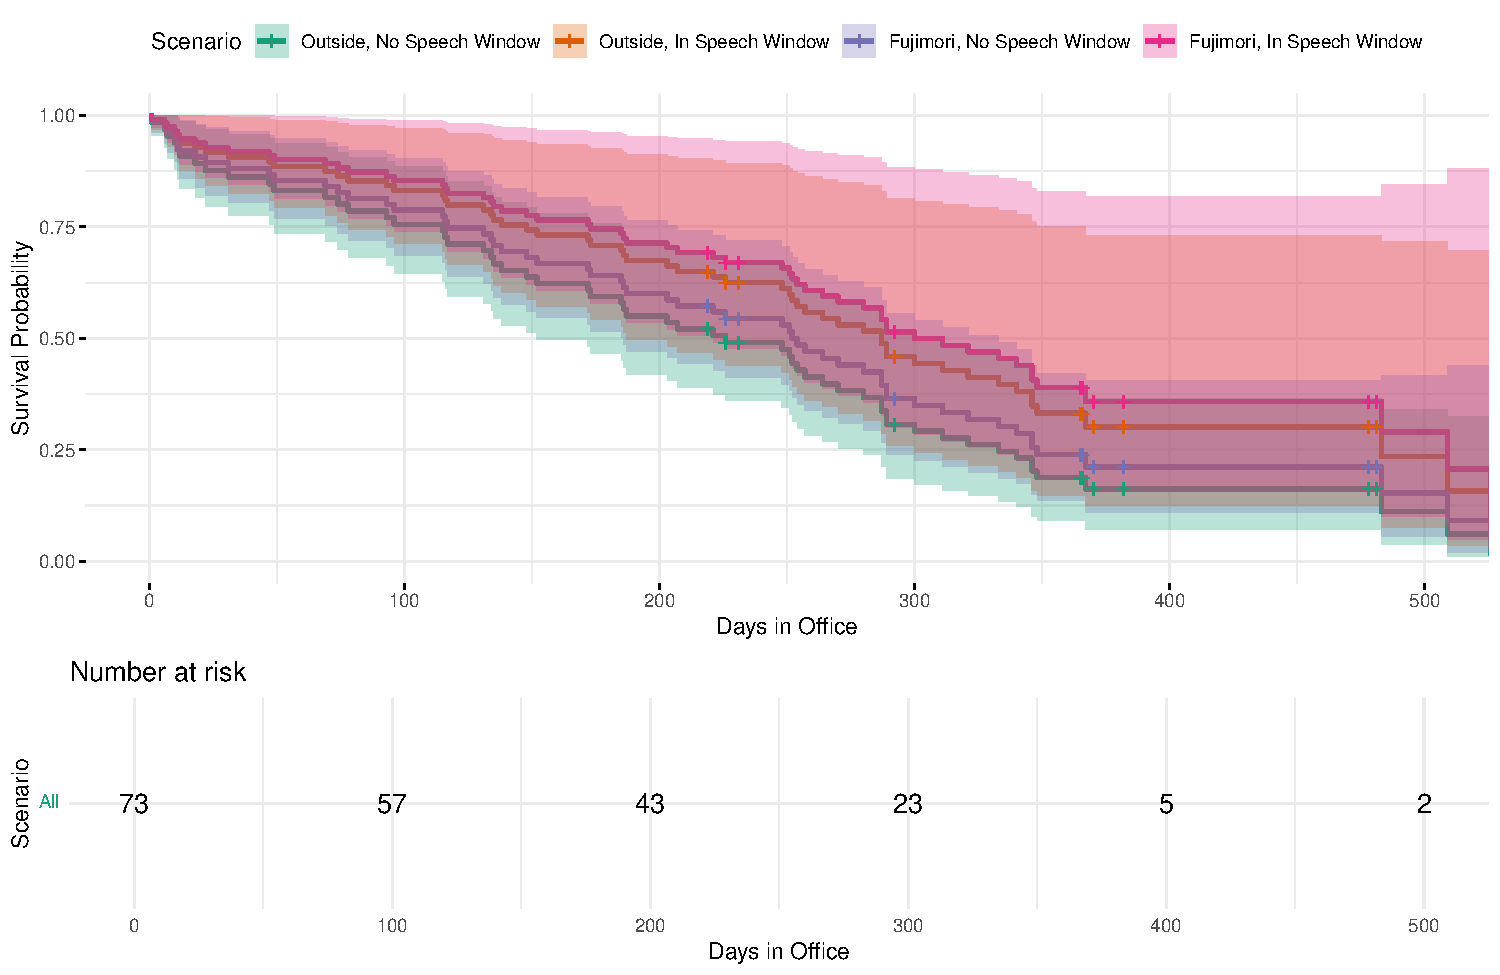
\includegraphics[width=0.85\textwidth]{combined_survival_plot.pdf}
% % \caption{Survival curves by scenario (Fujimori vs. Outside)}
% % \label{fig:survcurve}
% % \end{figure}
% 
% % \begin{sidewaysfigure}
%   \begin{figure}[ht]
%     \centering
%     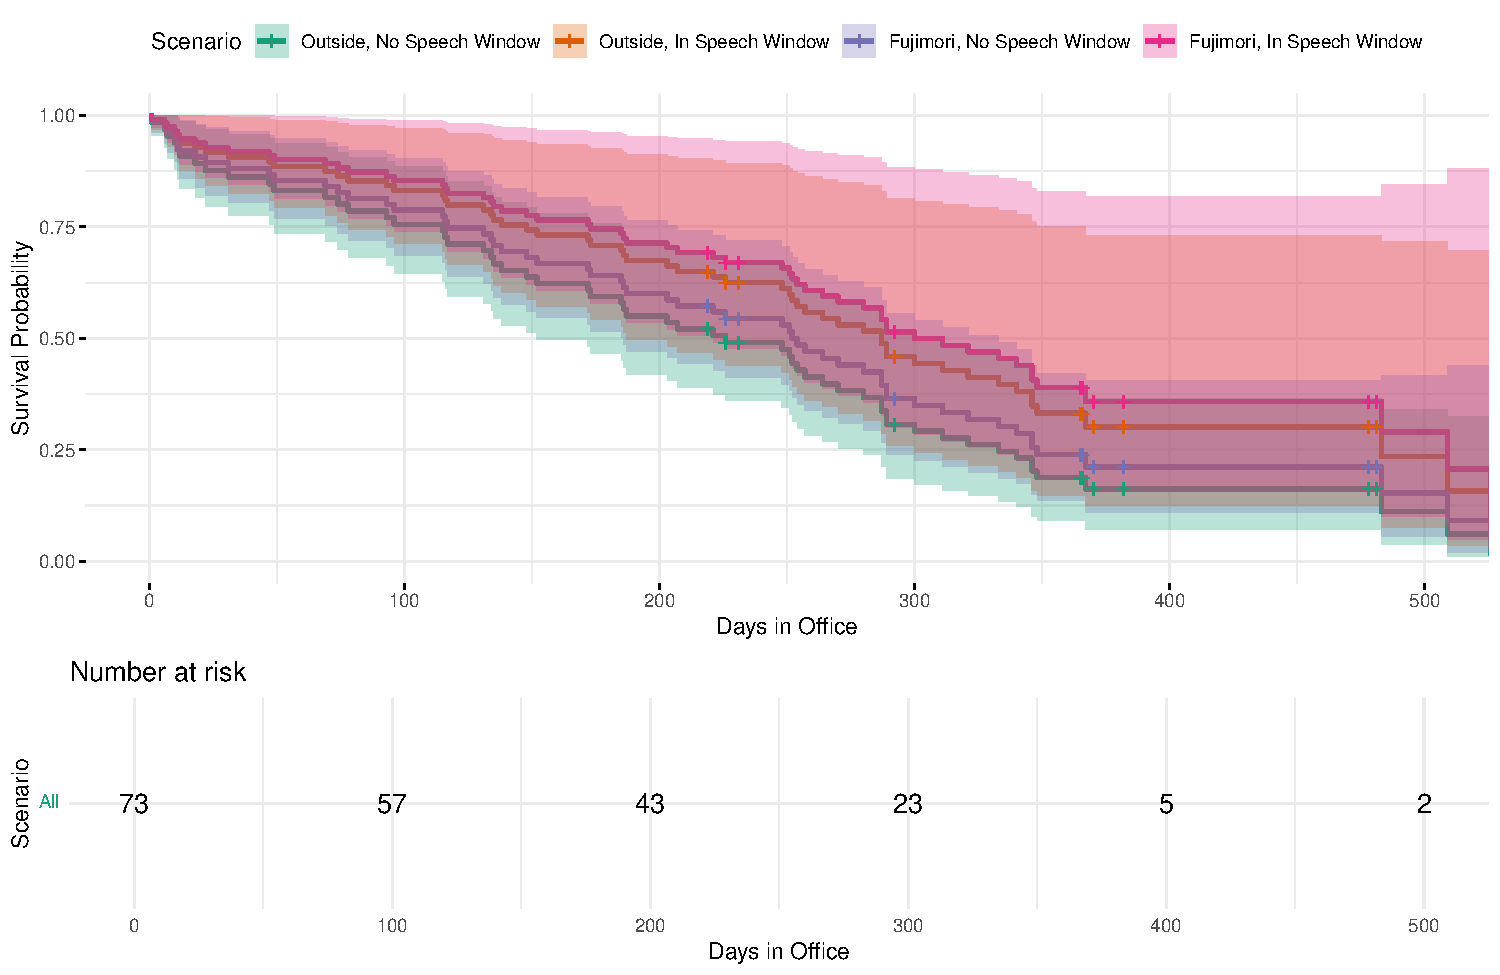
\includegraphics[width=\textwidth]{combined_survival_plot.pdf}
%     \caption{Estimated PCM survival curves under four scenarios: outside/in speech window and non‑Fujimori/Fujimori periods.}
%     \label{fig:survival_curves}
%   \end{figure}
% % \end{sidewaysfigure}
% 
% This plot shows four estimated survival curves—each with 95 \% confidence bands—derived from the simplified Cox model (no frailty) for combinations of the Fujimori regime dummy and the $\pm$ 45-day speech window:
% 
% \begin{itemize}
% \item Green (“Outside, No Speech Window”): PCM spells that start outside the speech window and outside the Fujimori period.
% 
% \item Orange (“Outside, In Speech Window”): Spells that start within ± 45 days of July 28 but outside Fujimori.
% 
% \item Blue (“Fujimori, No Speech Window”): Spells during Fujimori that start more than 45 days from the speech.
% 
% \item Pink (“Fujimori, In Speech Window”): Spells during Fujimori that start within the speech window.
% \end{itemize}
% 
% From this plot we can say that overall decline in survival. All curves drop from 1.0 toward 0 as days in office accumulate—by around 300 days only half of PCMs remain in office on average.
% 
% Regime effect (Fujimori vs. non-Fujimori): The two Fujimori curves (blue and pink) lie above their non-Fujimori counterparts, indicating longer average survival under Fujimori. For instance, at 200 days the survival probability is roughly 0.65 under Fujimori versus about 0.50 outside it.
% 
% Speech-window effect: Within each regime, the “in speech window” curve (orange and pink) tracks slightly above the “no speech window” curve (green and blue), suggesting a modest reduction in exit risk when a spell begins near the annual address date. This difference, however, is small relative to the CIs.
% 
% Precision declines over time: The shaded bands widen toward the right, reflecting increasing uncertainty as fewer spells survive into longer tenures. Beyond ~400 days, the confidence intervals become very wide, so point‐estimate differences at those durations are not very informative.
% 
% Number at risk: The table below shows how many intervals remain “at risk” at key time-points (0, 100, 200, … days). You start with 72 intervals (57 spells split at speech cut–points), dropping to just 2 intervals by ~500 days.
% 
% 
% Although the point estimates hint at better survival during Fujimori and slightly lower exit risk for spells initiated near the speech, these contrasts fall well within the wide confidence bands. This visual underscores why the minimal two-covariate model didn’t yield statistically significant regime or speech-window effects—and why adding the institutional (ENP), approval, and economic covariates is essential to sharpen the estimated drivers of PCM durability.
% 
% 
% 
% \section{Software and replication}
% 
% Models are estimated in R 4.3 using packages \emph{survival}, \emph{coxme}, and \emph{ggsurvfit}. All data and scripts are archived on Github
% 
% 
% \section{Conclusion}
% 
% \section{Apendixes}

% %%%%% adding bibliography
\bibliographystyle{apacite} %%style
\renewcommand{\refname}{Bibliography}
\bibliography{Premieres} %% filename

\end{document} %% nothing after here

